\begin{center}\large\textbf{Readings: 14.1-14.3 643-660}\\
\normalsize \end{center}
\large \hlinewd{2pt}
~\\
Thus far we've considered the means of our factors as the main things of interest (called fixed factors).  Sometimes we won't actually be interested in the mean of a factor but rather that factor's variability.  Random effects models allow for this type of inference.\\

\textbf{Example where a random factor is of interest.}
\begin{itemize}
\item Consider a genetics study with beef animals.  Response = birthweight $Y$ ($lbs$).
\item $t=5$ sires (male cows), each mated to a separate group of $n=8$ dams (female cows).
\item $N=40$, completely randomized design. 
\item Interest is in variability in birth rate based on sires.
\end{itemize}
\begin{center}
\begin{tabular}{cc|cccccccc|c|c}
\multicolumn{12}{c}{Birthweights} \\
Sire \# & Level & \multicolumn{8}{c|}{Sample} & $\tmean{i}$ & $s_i$ \\ \hline
177 & 1 & 61 & 100 & 56 & 113 & 99 & 103 & 75 & 62 & 83.6 & 22.6 \\
200 & 2 & 75 & 102 & 95 & 103 & 98 & 115 & 98 & 94 & 97.5 & 11.2\\
201 & 3 & 58 & 60  & 60 & 57 & 57 & 59 & 54 & 100 &  63.1 & 15.0\\
202 & 4 & 57 & 56  & 67 & 59 & 58 & 121 & 101 & 101& 77.5 & 25.9\\
203 & 5 & 59 & 46  & 120 & 115 & 115 & 93 & 105 & 75&91.0 & 28.0 \\ \hline 
\end{tabular}
\end{center}
What statistical model is appropriate for these data?  \\~\\
A: One-way `fixed' effects model?
$$ Y_{ij} = \underbrace{\mu}_{\text{fixed}} + \underbrace{\tau_i}_{\text{fixed}} + \underbrace{E_{ij}}_{\text{random}}$$
where $\tau_i$ denotes the difference between the mean birthweight of population of offspring from sire $i$ and $\mu$, mean of whole population.\\~\\
We don't really care about these 5 sires, but interest is more in the entire population of possible sires.  Here \textbf{sire is a random effect}.

\newpage

\begin{center}
Flow chart for identifying a factor as fixed or random.\\
\begin{tabular}{l| c c}
& Random & Fixed \\ \hline
Levels \\
- selected from conceptually $\infty$ popn of & X & \\
collection of levels & & \\
- finite number of possible  levels & & X \\
\\ \hline
Another expt & & \\
- would use same levels & & X \\
- would involve new levels sampled & X & \\
from same population \\
\\ \hline
Goal  & & \\
- estimate varcomps & X & \\
- estimate longrun means & & X\\
\\ \hline
Inference & & \\
- for these levels  used in this expt & & X\\
- for the population of levels & X & \\
\end{tabular}
\end{center}
Contrast this situation with the binding fractions example.  Why not model antibiotic effects random?  Why fixed?\\~\\~\\~\\

\textbf{The One-Way random effects model (One-Way implies one factor)}
$$ Y_{ij} = \underbrace{\mu}_{\text{fixed}} + \underbrace{T_i}_{\text{random}} + \underbrace{E_{ij}}_{\text{random}}$$
where $i=1,2,\ldots,t$ (number of levels) and $j=1,\ldots,n$ (number of replicates).
\begin{itemize}
\item Assume $T_1,T_2,\ldots,T_t \iid N(0,\sigma_T^2)$
\item Assume $E_{11},\ldots,E_{tn} \iid N(0,\sigma^2)$
\item Assume $T_1,T_2,\ldots,T_t$ independent of $E_{11},\ldots,E_{tn}$
\end{itemize}
Notation:
\begin{itemize}
\item $T_1,T_2,\ldots$ denote {\em random} effects, drawn from some population of interest. \\For beef animal genetic study, with $t=5$ and $n=8$, the random effects $T_1,T_2,\ldots,T_5$ reflect sire-to-sire variability.  
\item $\sigma_T^2$ and $\sigma^2$ are called the \textbf{variance components}
\item Conceptually different from one-way fixed effects model, but analysis is equivalent!
\end{itemize}

\newpage 

For random effects model we now have:
$$E(Y_{ij})=E(\mu+T_i+E_{ij})=E(\mu)+E(T_i)+E(E_{ij})=\mu + 0 + 0 =\mu$$
and
$$Var(Y_{ij})=Var(\mu+T_i+E_{ij})=Var(T_i)+Var(E_{ij})+2cov(T_i,E_{ij})=\sigma^2_T+\sigma^2+0=\sigma^2_T+\sigma^2$$
\begin{itemize}
\item Two {\em components} to variability in data: $\sigma^2, \sigma_T^2$
\end{itemize}~\\

ANOVA table for One-Way Random effects model is the same as the One-Way Fixed effects model!
\begin{center}
\begin{tabular}{cccc}
Source & SS & df & MS  \\ \hline
Treatment & $SS(Trt)$ & $t-1$ & $MS(Trt)$  \\
Error & $SS(E)$ & $N-t$ & $MS(E)$  \\
Total & $SS(Tot)$ & $N-1$ & \\ \hline
\end{tabular}
\end{center}
~\\
Only difference is the expected values of the Mean Squares:
\begin{itemize}
\item Expected mean square for error = $E(MS(E))=\sigma^2$
\item Expected mean square for treatment 
\begin{itemize}
\item For random effects model = $E(MS(Trt))=\sigma^2+n\sigma^2_T$\\
\item For fixed effects model = $E(MS(Trt))=\sigma^2+\frac{n}{t-1}\sum_{i=1}^{t}\tau_i^2$\\
\end{itemize}
\end{itemize}


\textbf{Main hypothesis of interest for One-Way random effects model:}
$$H_0:\sigma^2_T=0~~~~~vs.~~~~~~H_A:\sigma^2_T>0$$
If $H_0$ is true then
$$F=\frac{MS(Trt)}{MS(E)}\mbox{ will be approximately }\frac{\sigma^2+0}{\sigma^2}=1$$
If $H_0$ is false then
$$F=\frac{MS(Trt)}{MS(E)}\mbox{ will be greater than }1$$
Compare observed F to $F(t-1,N-t,\alpha)$.  Again, same as One-Way fixed effects ANOVA model.\\~\\~\\

\newpage

\textbf{Estimating parameters of One-Way random effects model:}\\
Estimate of $\mu$ is still
$$\hat\mu = \gmean$$
Estimate of $\sigma^2$ is still
$$\hat\sigma^2 = MS[E] $$
To estimate $\sigma^2_T$ we can 'equate mean squares'.  We know $E(MS(Trt))=\sigma^2+n\sigma^2_T$.  For large samples $MS(Trt)$ will be 'close' to $E(MS(Trt))$, so
$$\hat\sigma_T^2 = \frac{MS[T]-MS[E]}{n}$$
~\\~\\
For sires data, $\gmean=82.6$ and 
\begin{center}
\begin{tabular}{ccccc}
Source & SS & df & MS & Expected MS \\ \hline
Sire & 5591 & 4 & 1398 & $\sigma^2 + 8 \sigma_T^2$ \\
Error & 16233 &35 & 464 & $\sigma^2$  \\
Total & 21824 & 39 & &  \\ \hline
\end{tabular}
\end{center}
~\\~\\
Therefore, $\hat\mu = 82.6$, $\hat\sigma^2 = 464 (lbs^2)$, and $\hat\sigma_T^2 = \frac{1398-464}{8} = 117 \ (lbs^2)$.\\~\\
Note: If you get an estimated $\sigma^2_T$ that is negative, it should be set to zero.\\~\\~\\
\textbf{Testing a variance component - $H_0: \sigma_T^2=0$}\\
Recall that $\sigma_T^2 = \Var(T_i) $, the variance among the population of treatment effects.
$$ F=\frac{MS[T]}{MS[E]} $$
reject $H_0$ at level $\alpha$ if $F > F(\alpha,t-1,N-t)$
For the sires, 
$$ F=\frac{1398}{464} = 3.01 > 2.64 = F(0.05,4,35) $$ 
so $H_0$ is rejected at $\alpha=0.05$.  (The $p$-value is 0.0309)\\~\\
Q: ``Isn't this just just like the $F$-test for one-way ANOVA with {\em fixed} effects?"\\
A: ``Yes."

\newpage

\textbf{Specific questions pertaining to this study:}\\
Consider the birthweight of a randomly sampled calf.
\begin{enumerate}
\item What is the estimated variance of such a calf?\\~\\~\\~\\~\\~\\
\item Estimate the proportion of this variation that is due to the sire effect.\\~\\~\\~\\~\\~\\
\item Estimate the proportion of this variation that is not due to the sire effect.
\end{enumerate}

\newpage

\textbf{Other quantities of interest in random effects models:}\\~\\
\textbf{Coefficient of variation} (CV): 
$$ CV(Y_{ij}) = \frac{\sqrt{\Var(Y_{ij})}}{|E(Y_{ij}|} = \frac{\sqrt{\sigma_T^2 + \sigma^2}}{|\mu|}$$~\\
Note: this is {\em not} estimated by {\tt Coeff Var} in PROC GLM output.\\~\\~\\

\textbf{Intraclass correlation coefficient:} ($\rho_I$)
$$ \rho_I = \frac{\Cov(Y_{ij},Y_{ik})}{\sqrt{\Var(Y_{ij})\Var(Y_{ik})}}= \frac{\sigma_T^2}{\sigma_T^2 + \sigma^2}$$

\begin{itemize}
\item Interpretation: the correlation between two responses receiving the same level of the random factor.
\item Bigger values of $\rho_I$ correspond to larger random treatment effects.
\end{itemize}
~\\~\\
For the sires data,
$$\widehat{CV}  =  \frac{\sqrt{117 + 464}}{82.6} = 0.29 $$
$$\hat\rho_I = \frac{117}{117+464} = 0.20$$ 

Interpretations:
\begin{itemize}
\item The estimated standard deviation of a birthweight, 24.1 (lbs), is $29\%$ of the estimated mean birthweight, $82.6$.
\item The estimated correlation between any two calves with the same sire for a male parent, or the estimated {\em intrasire} correlation
coefficient, is $0.20$
\end{itemize}

\newpage

\textbf{Using Proc GLM and Proc Mixed for random effects models:}\\~\\
\begin{small}
\begin{verbatim}
proc glm data=sires;                 
class sire;                          
model BirthWeight=Sire;              
random Sire;                         
run;                                 
\end{verbatim}
\end{small}

\begin{center}
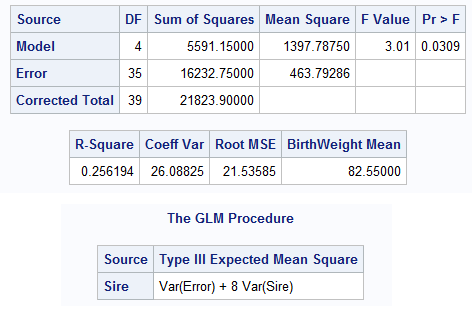
\includegraphics[scale=0.8]{Sire1}
\end{center}

\begin{small}
\begin{verbatim}
proc mixed data=sires method=type3;                 
class sire;                          
model BirthWeight=;              
random Sire;                         
run;                                 
\end{verbatim}
\end{small}

\begin{center}
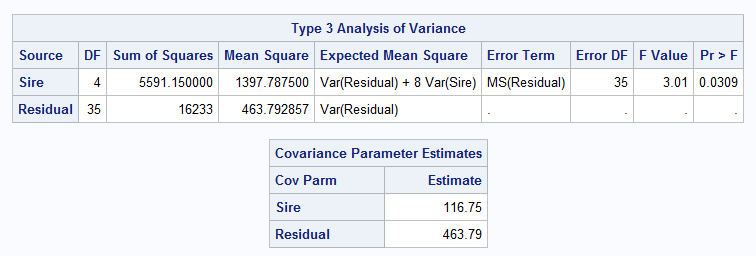
\includegraphics[scale=0.8]{Sire2}
\end{center}

(Note:  $\sigma^2=${\tt Var(Error)}  and $\sigma_T^2=${\tt Var(sire)}.)  

\newpage

\newpage
\textbf{Interval Estimation of $\mu$}\\~\\
A $100(1-\alpha)\%$ confidence interval for $\mu$ can be easily derived by consideration of $SE(\bar{Y}_{++})$:
\beq{
\bar{Y}_{++} &=& \frac{1}{N}\sum_{i=1}^t \sum_{j=1}^n Y_{ij} \\
&=& \frac{1}{N}\sum_{i=1}^t \sum_{j=1}^n (\mu + T_i + E_{ij}) \\
&=& \mu + \bar{T}_{+} + \bar{E}_{++}}
where $\bar{T}_{+}=(T_1 + \cdots + T_t)/t$ and $\bar{E}_{++}=(\sum \sum E_{ij})/N$,
so that
\beq{
\Var(\bar{Y}_{++}) &=& \Var(\bar{T} + \bar{E}_{++}) \\
&=& \frac{\sigma_T^2}{t} + \frac{\sigma_2}{nt} \\
&=& \frac{1}{nt}(n \sigma_T^2 + \sigma^2) \\
&=& \frac{1}{nt}E(MS[T]).}
If the data are normally distributed, then 
$$\frac{\bar{Y}_{++}-\mu}{\sqrt{\frac{MS[T]}{nt}}} \sim t_{t-1}$$
and a $100(1-\alpha)\%$ confidence interval for $\mu$ given by
$$\bar{Y}_{++} \pm t(\alpha/2,t-1) \sqrt{\frac{MS[T]}{nt}}$$

Sires data: $\gmean=82.6, MS[T]=1398, nt=40.$ 
Critical value $t(0.025,4)=2.78$ yields the 95\% CI
$$82.6 \pm 2.78 (5.91) \ \mbox{ or } \ (66.1,99.0).$$
We are 95\% confident the true mean birthweight is between 66.1 and 99.0 lbs.\\~\\
By adding in the statement 'estimate 'mean' intercept 1/cl' to the proc mixed code we get (can use type3 or reml method)
\begin{center}
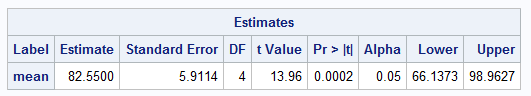
\includegraphics[scale=0.8]{Sire3}
\end{center}

\textbf{Interval estimation for variance components:}\\
The estimated residual variance component for the sire data was
$$\hat\sigma^2 = MS[E] = 464~lbs^2$$ 
A $100(1-\alpha)\%$ confidence interval for this variance component is given by 
$$ \left(\frac{(N-t)MS[E]}{\chi^2_{\alpha/2}}, \ \frac{(N-t)MS[E]}{\chi^2_{1-\alpha/2}}\right).$$ 
For the sire data and $\alpha=0.05$ this becomes,
$$\left(\frac{(40-5)464}{53.2} < \sigma^2 < \frac{(40-5)464}{20.6}\right) $$
$$\left(\frac{35}{53.2}464 < \sigma^2 < \frac{35}{20.6}464\right)$$
or $(305.2,789.5) lbs^2$\\
We are 95\% confident the true error variance is between 305.2 and 789.5 $lbs^2$.\\~\\
%For those interested, this is derived using 
%$$ (N-t)\frac{MS[E]}{\sigma^2} \sim \chi^2_{N-t}$$
%setting up the probability statement
%$$ 1 - \alpha = \Pr\left(\chi^2(1-\frac{\alpha}{2},N-t) < (N-t)\frac{MS[E]}{\sigma^2} < \chi^2(\frac{\alpha}{2},N-t)\right)$$
%Rearranging to get $\sigma^2$ in the middle yields the $100(1-\alpha)\%$ confidence interval for $\sigma^2$.\\~\\~\\

\textbf{Interval estimation for $\sigma_T^2$}\\
The estimated variance component for the random sire effect was $\hat\sigma_T^2 = 117$.\\
A $100(1-\alpha)\%$ confidence interval for $\sigma^2_T$ is given by 
$$ \left(\frac{\widehat{df}\hat\sigma_T^2}{\chi^2_{\alpha/2,\widehat{df}}}, \ \frac{\widehat{df}\hat\sigma_T^2}{\chi^2_{1-\alpha/2,\widehat{df}}}\right)$$ 
where 
$$\widehat{df} = \frac{(n \hat\sigma_T^2)^2}{\frac{MS[T]^2}{t-1} + \frac{MS[E]^2}{N-t}}$$
is the Satterthwaite approximation to the degrees of freedom.\\~\\
For the sire data,
$$ \widehat{df} = \frac{(8 \times 117)^2}{\frac{1398^2}{4}+\frac{464^2}{35}} = 1.76$$

Software must be used to obtain this non-integer degrees of freedom (using a table we'd have to round to the nearest integer):
$$ \chi^2_{0.975,1.76} = 0.029, \ \ \ \chi^2_{0.025,1.76} = 6.87 $$
yielding the $95\%$ confidence interval
$$ \left(\frac{1.76 (117)}{6.87} \ \frac{1.76 (117)}{0.29} \right)=(30,7051)$$
We are 95\% confident the variance between sires is between 30 and 7051 $lbs^2$.

\newpage
To get these two intervals in SAS we need to use proc mixed with `reml' estimation rather than type3.\\~\\
\begin{small}
\begin{verbatim}
proc mixed data=sires method=reml cl;
class sire; 
model BirthWeight=; 
random Sire; 
run;
\end{verbatim}
\end{small}

\begin{center}
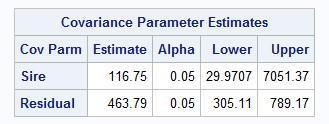
\includegraphics[scale=0.9]{Sire4}
\end{center}

Note:  The estimates of the variance components using type3 and reml estimation match here, this is not always the case.\\~\\~\\
\textbf{Confidence interval for $\rho_I$:}\\
A $100(1-\alpha)\%$ confidence interval for $\rho_I$ is given by
$$\left(\frac{F_{obs}-F_{\alpha/2}}{F_{obs}+(n-1)F_{\alpha/2}},\frac{F_{obs}-F_{1-\alpha/2}}{F_{obs}+(n-1)F_{1-\alpha/2}}\right) $$
where $F_{\alpha/2}=F(\frac{\alpha}{2},t-1,N-t)$ and $F_{obs}$ is the observed $F$-ratio for treatment effect from the ANOVA table.\\~\\
For the sires, $F_{obs}=3.01$ and $F_{0.025}=3.179, F_{0.975} = 0.119$.\\
The formula gives $(-0.01,0.75)$.  \\~\\
We are 95\% confident the intraclass correlation coefficient is between -0.01 and 0.75.

%These formulas arrived at via some distributional results:
%\begin{itemize}
%\item $(t-1)\frac{MS[T]}{\sigma^2+n\sigma_T^2} \sim \chi^2_{t-1}$
%\item $(N-t)\frac{MS[E]}{\sigma^2} \sim \chi^2_{N-t}$
%\item $MS[T]$ and $MS[E]$ are independent 
%\item Ratio of independent $\chi^2$ RVs divided by $df$ has an $F$ distribution
%\item $$\frac{\frac{MS[T]}{\sigma^2+n\sigma_T^2}}{\frac{MS[E]}{\sigma^2}} \sim F_{t-1,N-t}$$
%\item $$\left(\frac{MS[T]}{\sigma^2+n\sigma_T^2}\right)/\left(\frac{MS[E]}{\sigma^2}\right) \sim F_{t-1,N-t}$$
%(which explains the $F$ test for $H_0: \sigma_t^2=0$)
%\item Rearranging the probability statement below
%$$ 1-\alpha = \Pr\left(F(1-\frac{\alpha}{2},t-1,N-t) < \frac{\frac{MS[T]}{\sigma^2+n\sigma_T^2}}{\frac{MS[E]}{\sigma^2}} < F(\frac{\alpha}{2},t-1,N-t)\right) $$
%so that $\rho_I$ gets left in the middle yields the confidence interval
%yields the c.i. at the top o' the page.
%$$\frac{F_{obs}-F_{1-\alpha/2}}{F_{obs}+(n-1)F_{1-\alpha/2}} < \rho_I <
%\frac{F_{obs}-F_{\alpha/2}}{F_{obs}+(n-1)F_{\alpha/2}} $$
%\end{itemize}



\newpage
\textbf{Review of one-way random effects ANOVA}\\~\\

Model:
$$ Y_{ij} = \underbrace{\mu}_{\text{fixed}} + \underbrace{T_i}_{\text{random}} 
+ \underbrace{E_{ij}}_{\text{random}} \text{ for }i=1,2,\ldots,t\mbox{ and }
j=1,\ldots,n$$
with
%\begin{itemize}
%\item $T_1,T_2,\ldots,T_t \iid N(0,\sigma_T^2)$ independent of $E_{11},\ldots,E_{tn} \iid N(0,\sigma^2)$
%%\item $T_1,T_2,\ldots,T_t$ independent of $E_{11},\ldots,E_{tn}$
%\end{itemize}
$$T_1,T_2,\ldots,T_t \iid N(0,\sigma_T^2)\ \mbox{ independent of }\ E_{11},\ldots,E_{tn} \iid N(0,\sigma^2)$$
\bigkn
Remarks:
\begin{itemize}
\item
($T_1,T_2,\ldots$ randomly drawn from pop'n of treatment
effects.)
\item Only three parameters: $\mu,\sigma,\sigma_T^2$
\item Several functions of these parameters of interest
\begin{itemize}
\item $CV(Y)=\frac{\sqrt{\sigma^2 + \sigma_T^2}}{\mu}$
\item $\rho_I=\mbox{Corr}(Y_{ij},Y_{ik})=\frac{\sigma_T^2}{\sigma^2 + \sigma_T^2}$
\end{itemize}
\item Two observations from same treatment group not independent
\end{itemize}
%Loads-of-fun 
Exercise: match up the formulas for confidence intervals
below with their targets, $\rho_I,\sigma^2,\sigma_T^2,\mu$: 
%\begin{center}
%\fbox{$\Gmean \pm t(0.025,t-1) \sqrt{\frac{MS[T]}{nt}}$}
%\end{center}
$$Y_{++} \pm t(0.025,t-1) \sqrt{\frac{MS[T]}{nt}}$$
$$\left(\frac{F_{obs}-F_{1-\alpha/2}}{F_{obs}+(n-1)F_{1-\alpha/2}},\frac{F_{obs}-F_{\alpha/2}}{F_{obs}+(n-1)F_{\alpha/2}} \right)$$
$$\left(\frac{(N-t)MS[E]}{\chi^2_{\alpha/2}},\frac{(N-t)MS[E]}{\chi^2_{1-\alpha/2}}\right)$$
$$\left(\frac{\widehat{df}\hat\sigma_T^2}{\chi^2_{\alpha/2,\widehat{df}}} ,\frac{\widehat{df}\hat\sigma_T^2}{\chi^2_{1-\alpha/2,\widehat{df}}} \right)$$

